\section{The \UWCQ{} evidence-audit stack}
\label{sec:framework}

\paragraph{C: strong classical control and retained core.}
A per-task value-minus-cost seed is improved by best legal one-coordinate moves until convergence. Cluster destroy/repair then exactly enumerates one three-task cluster (occasionally plus one external task) for 18 iterations and two restarts. This is motivated by adaptive large-neighborhood search~\citep{ropke2006alns}, but we call the implemented method \emph{cluster repair} to avoid implying a broad ALNS benchmark. Let $y^G,y^C$ be the greedy and cluster incumbents, $\Delta=S(y^C)-S(y^G)$, $d=|I|^{-1}\sum_i\ind[y_i^G\ne y_i^C]$, and $v_R$ restart-score variance. Classical ambiguity is
\begin{equation}
 a=\min\!\left\{1,,2.8d+5\left[\frac{\Delta}{\max(|S(y^C)|,1)}\right]_+ +4\frac{\sqrt{v_R}}{\max(|S(y^C)|,1)}\right\}.
 \label{eq:ambiguity}
\end{equation}
Clusters are ranked by their complementarity/penalty magnitudes plus disagreement; four task indices $I_4$ are retained. Every assignment in $\prod_{i\in I_4}D_i$ is evaluated exactly with $y^C$ fixed outside $I_4$. The strict set $\mathcal Z=\{z:F(z,y^C_{-I_4})=1\}$ has at most $3^4=81$ states. If empty, the lowest 20\% by an explicit violation score is retained and marked fallback, never relabeled feasible.

\paragraph{W, U and Q: matched distributions.}
The warm state $z_W$ is the retained state nearest the cluster incumbent, and the normalized initial amplitude is
\begin{equation}
 \langle z|\psi_0\rangle\propto\exp[-.35d_H(z,z_W)].
 \label{eq:warm}
\end{equation}
The retained graph connects states differing by one mode; isolated nodes connect to their nearest retained neighbor. With energy $E(z)=-S(z,y^C_{-I_4})$, standardized diagonal cost Hamiltonian $H_C$ and mixer $H_M=-A_{\mathcal Z}$, the simulated state is
\begin{equation}
 |\psi_p(\boldsymbol\gamma,\boldsymbol\beta)\rangle=\prod_{\ell=1}^{p}e^{-i\beta_\ell H_M}e^{-i\gamma_\ell H_C}|\psi_0\rangle.
 \label{eq:qaoa}
\end{equation}
The uniform comparator uses $P_U(z)=1/|\mathcal Z|$. QAOA uses exact noiseless statevector probabilities. Both are sampled with replacement for 128 matched-budget draws. Primary quantum evidence is optimum mass $p^\star=\sum_{z:E(z)=E_{\min}}P(z)$; first-hit draw $T$ is a sampling proxy with misses coded 129, not wall-clock runtime.

\begin{table}[t]
\centering
\caption{The \textsc{U--W--C--Q} layers and their evidentiary roles.}
\label{tab:uwcq}
\scriptsize
\begin{tabularx}{\linewidth}{@{}p{0.07\linewidth}p{0.20\linewidth}p{0.31\linewidth}X@{}}
\toprule
Layer & Implemented object & Formula / metric & Role \\
\midrule
U & Uniform retained-state sampler & $P_U(z)=1/|\mathcal Z|$; 128 draws & Uninformed feasible-set comparator. \\
W & ALNS-nearest warm state & $\psi_0(z)\propto e^{-0.35d_H(z,z_W)}$ & Biases initial amplitude toward the incumbent. \\
C & Greedy, cluster repair, exact core, verifier & $\Delta=S_C-S_G$, $d=n^{-1}\sum_i\mathbf1[y_i^G\ne y_i^C]$ & Builds incumbent/core and checks accepted assignments. \\
Q & Retained-graph statevector QAOA & $\prod_{\ell=1}^p e^{-i\beta_\ell H_M}e^{-i\gamma_\ell H_C}|\psi_0\rangle$ & Tests probability concentration, not runtime advantage. \\
\bottomrule
\end{tabularx}
\end{table}

\begin{figure}[t]
  \centering
  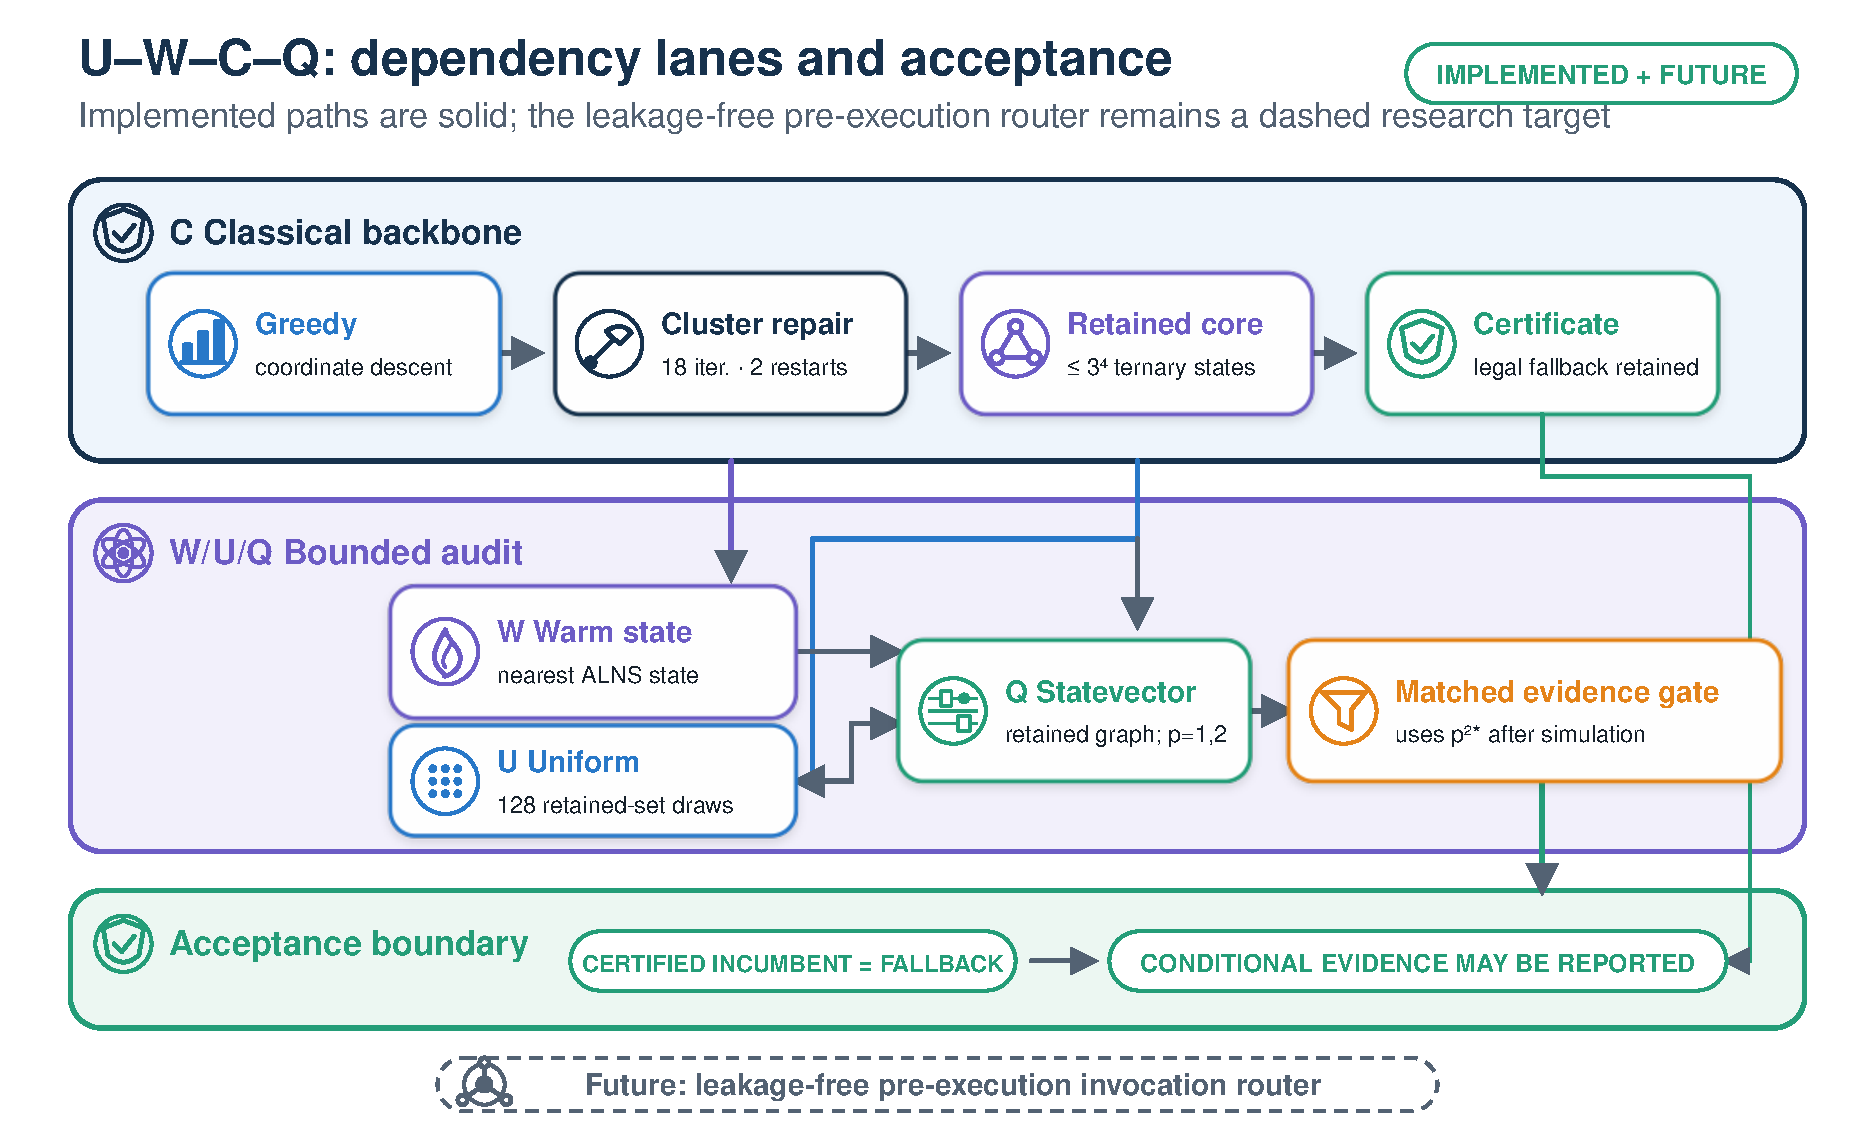
\includegraphics[width=\linewidth]{figs/fig3_uwcq_pipeline.pdf}
  \caption{Dependency lanes of \textsc{U--W--C--Q}. The classical backbone supplies the incumbent, retained core, and legal fallback; \textsc{W} and the retained set feed the bounded \textsc{U}/\textsc{Q} audit; the acceptance lane preserves classical certification. Because the evidence gate uses the simulated $p=2$ optimum mass, it is post-simulation and is not a cost-saving router. The dashed router is future work.}
  \label{fig:uwcq}
\end{figure}


\paragraph{Evidence gate and certificate.}
The frozen gate is
\begin{equation}
 g=F_{I_4}\land(a\ge.08)\land\left(p_2^\star\ge\max\{.18,1.4p_U^\star\}\right)\land(\Delta>10^{-6}\lor d\ge.05).
 \label{eq:gate}
\end{equation}
Crucially, $g$ consumes $p_2^\star$; it is a \emph{post-simulation evidence-eligibility indicator}, not a pre-execution invocation router. It therefore cannot reduce quantum cost. The final operational object in the present experiment remains the classically evaluated cluster-repair incumbent; the quantum branch audits the retained distribution and does not implement production candidate selection. Appendix~\ref{app:uwcq} provides the full formula glossary.
